\documentclass{beamer}
\usepackage{coloremoji}
\usecolortheme[dark,accent=cyan]{solarized}

\beamertemplatenavigationsymbolsempty

\usepackage{graphicx}
\usepackage{hyperref}
\usepackage{colortbl, xcolor}
\usepackage{booktabs}
\usepackage{varwidth}
\usepackage{hyperref}

\usepackage{tikz}
\usetikzlibrary{positioning,calc}
\usetikzlibrary{automata}
\usepackage{pstricks}
\usepackage{minted}

\definecolor{DarkGray}{gray}{0.1}
\definecolor{DarkGray}{gray}{0.1}
\usemintedstyle{native}

\title{Accessing open research literature with Python}
\author{@NikoletaGlyn}
\date{ }
\institute[]
{
\begin{center}
    
\includegraphics[width=.15\textwidth]{static/pycon-namibia.png}
\end{center}
}

\begin{document}

\frame{\titlepage}

\begin{frame}
    \begin{center}
    
\includegraphics[width=0.24\textwidth]{static/cardiff_uni_logo.jpg}\hspace{10pt}
    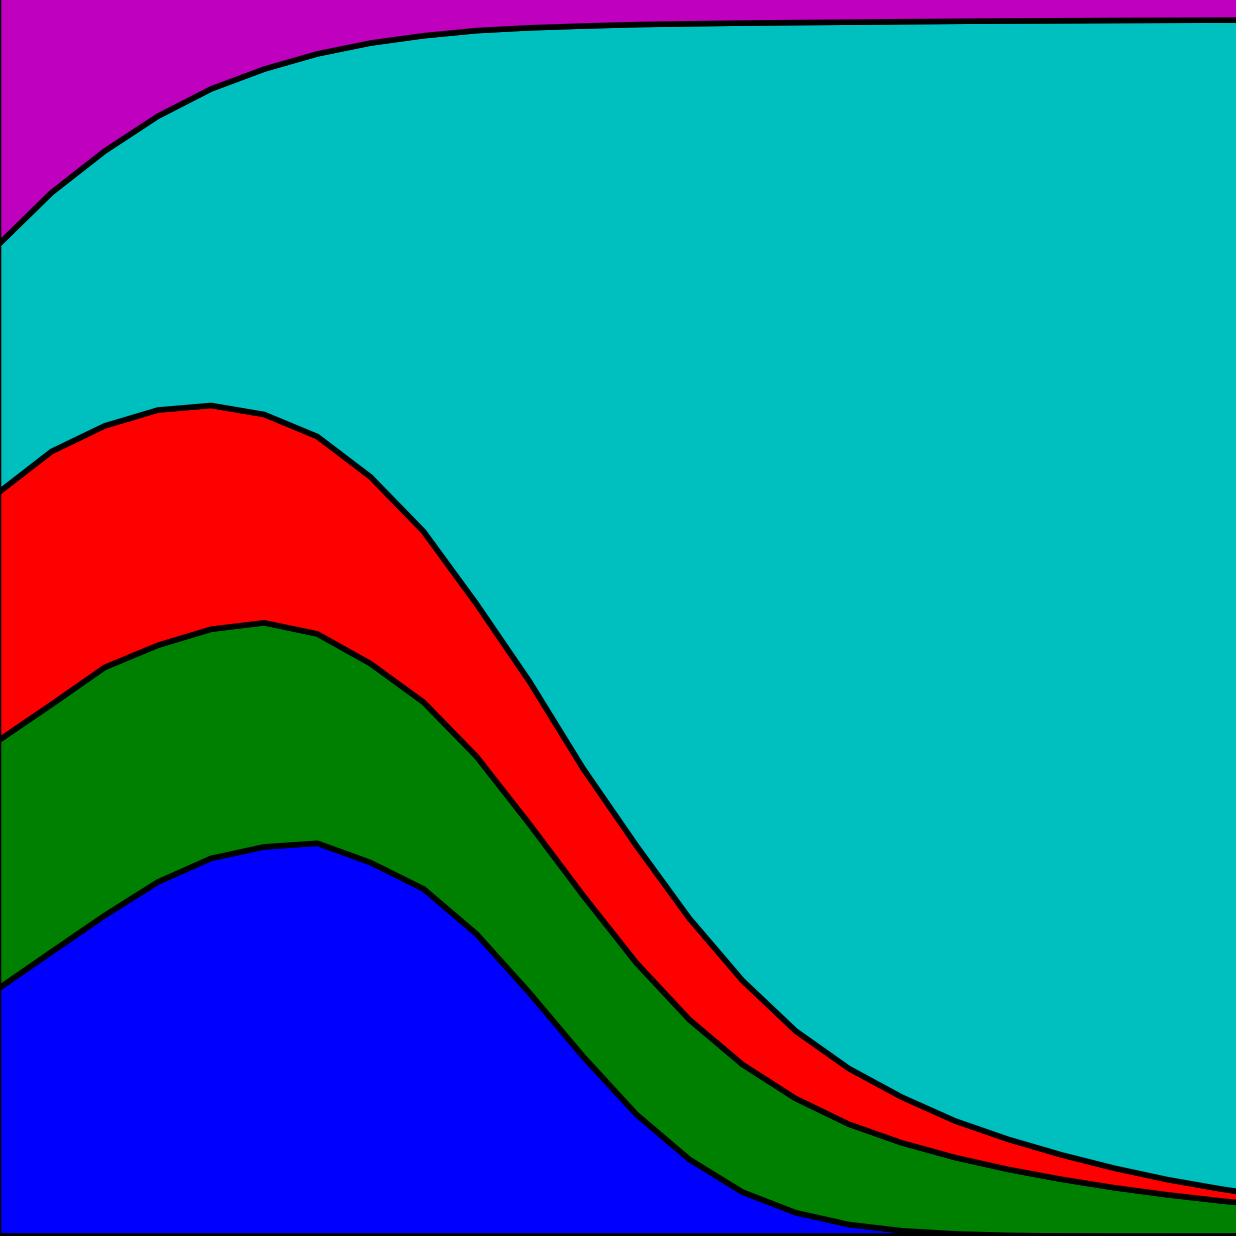
\includegraphics[width=0.24\textwidth]{static/axelrod-logo.png}\vspace{10pt}

    
\includegraphics[width=0.24\textwidth]{static/ssi-logo.png} \hspace{10pt}
    
\includegraphics[width=0.24\textwidth]{static/phoenix-logo.jpg}
    \vspace{10pt}
    \end{center}
\end{frame}

\begin{frame}
\begin{center}
\huge{The illustrated guide to a Ph.D.} \\
\vspace{10mm}
\large{Matt Might} \\
\vspace{10mm}
\tiny{http://matt.might.net/articles/phd-school-in-pictures/}
\end{center}
\end{frame}

\begin{frame}
    \begin{center}
    \tikzstyle{arrow} = [thick,->,>=stealth]

\begin{center}
\begin{tikzpicture}

\draw (0, 0) circle (3cm);
\draw[blue!70,fill=blue!70] (0, 0) circle (0.5cm);
\draw[line width=1mm, yellow!70](0, 0) circle (0.8);
\draw [arrow, line width=0.5mm, red!70] (0.5, 0.7) -- (0.7, 1);
\draw [arrow, line width=0.5mm, red!40] (0.5, 0.7) -- (0.7, 1);
\draw [arrow, line width=0.5mm, red!60] (0.7, 1) -- (.95, 1.4);

\draw [arrow, line width=0.5mm, red!80] (0.95, 1.4) -- (1.67, 2.5);

\end{tikzpicture}
\end{center}
    \end{center}
\end{frame}

\begin{frame}
\begin{figure}[width=\textwidth]
    \tikzstyle{arrow} = [thick,->,>=stealth]

\begin{center}
\begin{tikzpicture}\

\node[align=center, text=yellow!79] (c1) {\Large{WRITE}};
\begin{scope}
\node[align=center,text=yellow!79, right=4cmof c1] (c2) { \Large{REVIEW}};
\node[align=center,text=yellow!79, below=2cmof c2] (c3) {\Large{PUBLISH}};
\end{scope}

\draw [arrow] (c1) -- (c2);
\draw [arrow] (c2) -- (c1);
\draw [arrow] (c2) -- (c3);
\end{tikzpicture}
\end{center}
\end{figure}
\end{frame}

\begin{frame}
\begin{center}
    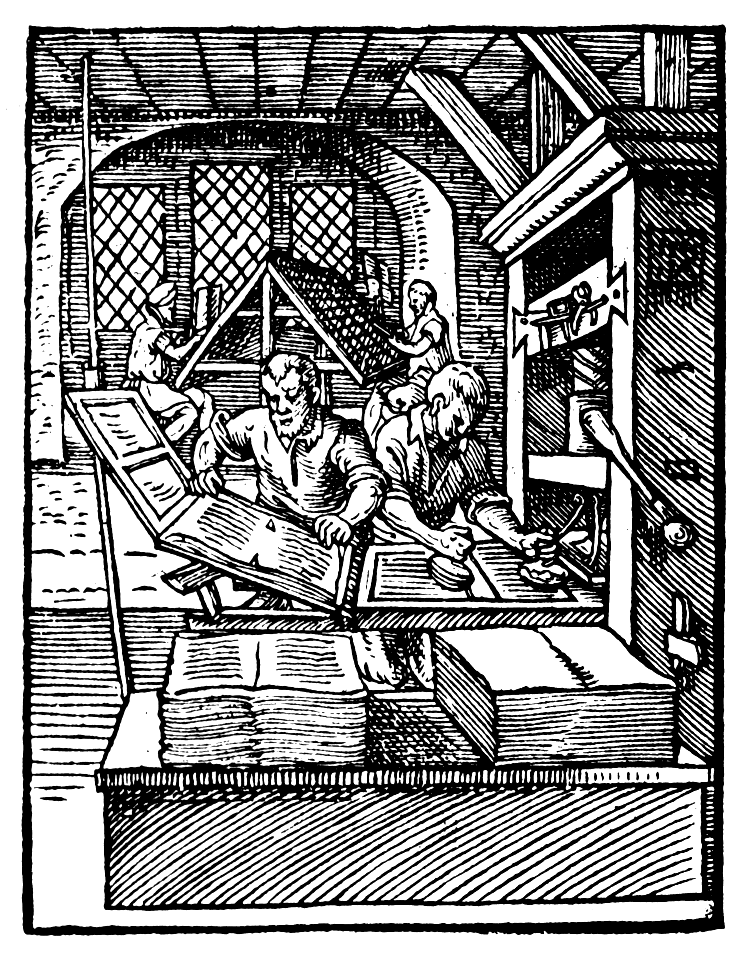
\includegraphics[width=0.5\textwidth]{static/printing.png} \\
    \small{1436}
\end{center}
\end{frame}

\begin{frame}
    \begin{center}
    \begin{tikzpicture}
   \foreach \x in {0,60,...,300}
      \node at (\x:2.5) {%
         \Huge{💻}} ;
\end{tikzpicture} \\
    \small{1980s}
    \end{center}
\end{frame}

\begin{frame}
\begin{center}
    \Huge{NAMIBIA}
\end{center}
\end{frame}

\begin{frame}
\begin{center}
    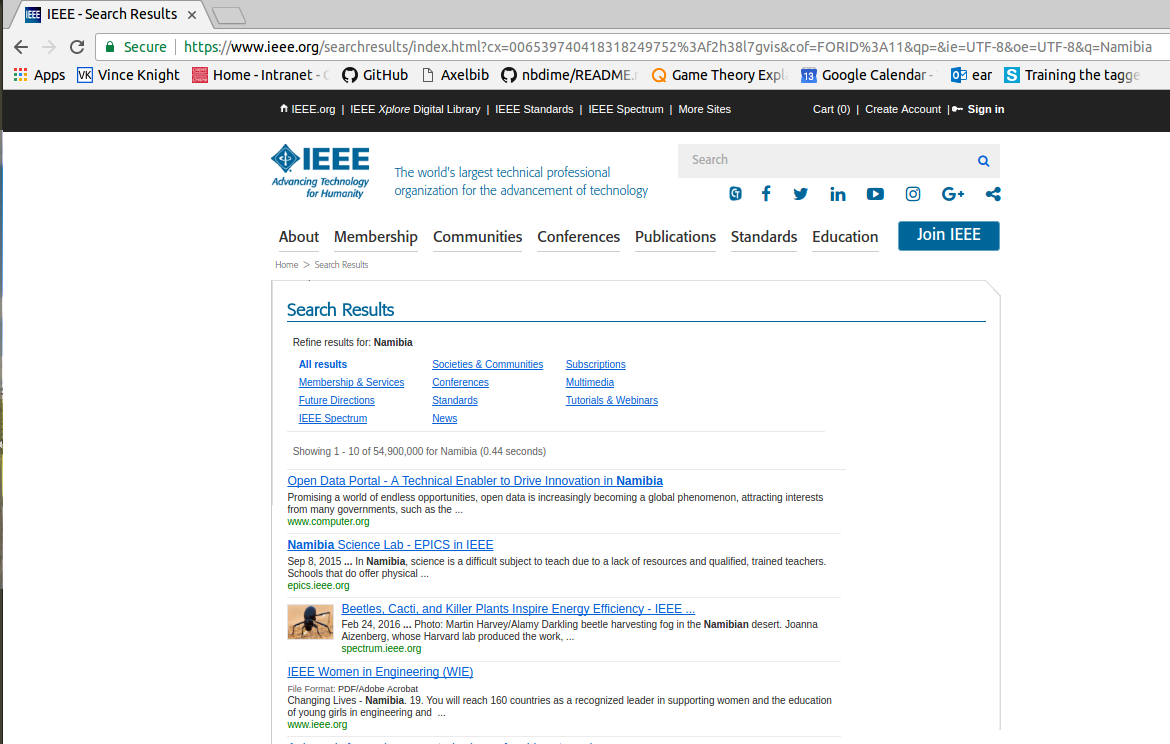
\includegraphics[width=1\textwidth]{static/ieee_manual.png}
\end{center}
\end{frame}

\begin{frame}
\begin{center}
\color{yellow!79}\Large{$0.5 min + \textrm{100} \times 1.5 min + 10 \times (0.5
\textrm{min})= 155.5 \textrm{min} \Rightarrow 2 \textrm{h} \textrm{ and } 35.5
\textrm{min}$}
\end{center}
\end{frame}

\begin{frame}
\begin{center}
\Huge{API}
\end{center}
\end{frame}

\begin{frame}[fragile]
    \begin{center}
    \textbf{QUERY} \\
    \vspace{3mm}
    \small{\url{http://ieeexplore.ieee.org/gateway/ipsSearch
    .jsp?ti=Namibia&hc=100}} \\
    \pause
    \vspace{10mm}
    \small{\url{http://api.plos.org/search?q=title:Namibia&rows=100}} \\
    \pause
    \vspace{10mm}
    \small{\url{http://www.nature.com/opensearch/request?queryType=cql&query=dc
    .title%20adj%20Namibia&maximumRecords=100}} \\
    \small{...}
    \end{center}
\end{frame}

\begin{frame}[fragile]
\begin{figure}
    \small{SCREENSHOT}
 \end{figure}
\end{frame}

\begin{frame}
\begin{center}
\color{yellow!79}\Large{$15 \textrm{min} + 1 \textrm{min} + 50 \textrm{min} =
66 \textrm{min} \Rightarrow 1\textrm{h} \textrm{ and } 6 \text{min}$}
\end{center}
\end{frame}

\begin{frame}
    \begin{center}
    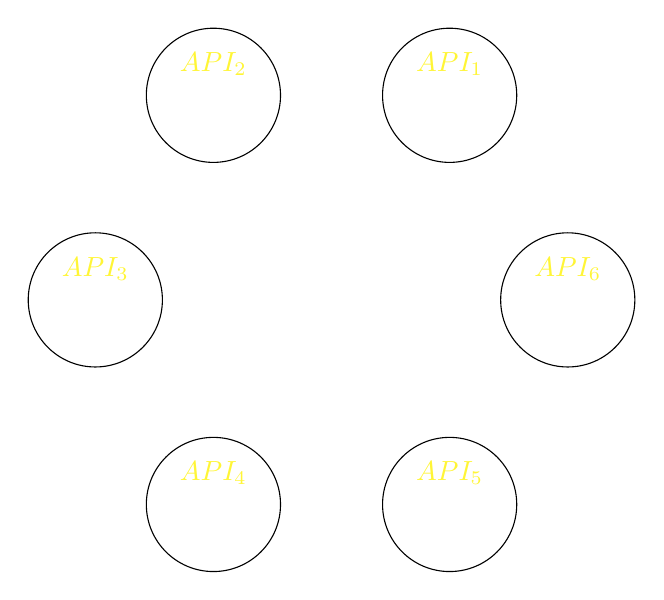
\begin{tikzpicture}

\foreach \phi in {1,...,6}{
    \node[state, align=center] (v_\phi) at (360/6 * \phi:3cm) {\color{yellow!79}$API_\phi$ \\\color{white!79}\tiny{Query}
    \\ \color{white!79}\tiny{XML}};
}
\end{tikzpicture}
    \end{center}
\end{frame}
\begin{frame}
    \begin{center}
    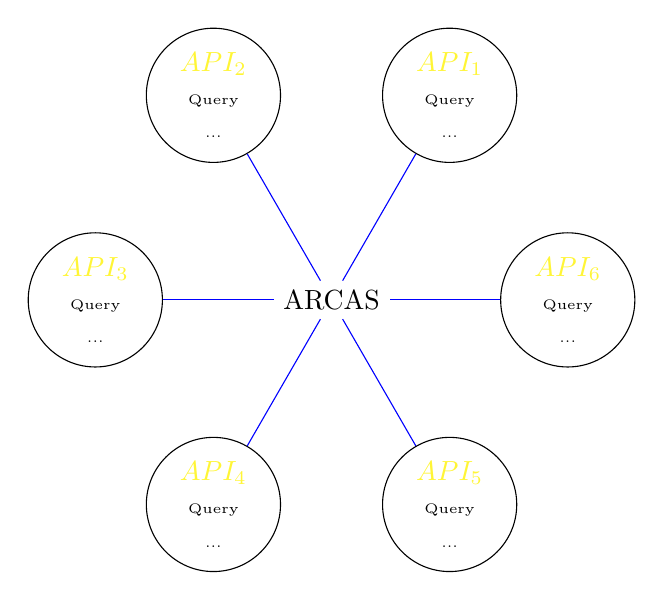
\begin{tikzpicture}

    \node (center) at (0,0) {ARCAS};
\foreach \phi in {1,...,6}{
    \node[state, align=center] (v_\phi) at (360/6 * \phi:3cm) {\color{yellow!79}$API_\phi$ \\ \tiny{Query} \\ \tiny{...}};
         \draw[blue] (v_\phi) -- (center);
}
\end{tikzpicture}
    \end{center}
\end{frame}

\begin{frame}[fragile]
    \begin{minted}
    [
    framesep=4mm,
    baselinestretch=1.2,
    bgcolor=DarkGray,
    fontsize=\Large,
    ]
    {python}
pip install arcas
    \end{minted}
\end{frame}

\begin{frame}[fragile]
    \begin{minted}
    [
    framesep=4mm,
    baselinestretch=1.2,
    bgcolor=DarkGray,
    fontsize=\tiny,
    ]
    {python}
import pandas as pd
from arcas import *

def get_arguments(word, start, count):
    arguments = {'-a': None, '-t': word, '-s': start,
                 '-r': count, '-y': None, '-b': None}
    return arguments

def main_program(arguments):
    parameters = pp.parameters_fix(arguments=arguments)
    url = pp.create_url_search(parameters=parameters)
    response = pp.make_request(url)
    root = pp.get_root(response)
    article = pp.parse(root)
    return article, url
    \end{minted}

    \begin{minted}
    [
    framesep=4mm,
    baselinestretch=1.2,
    bgcolor=DarkGray,
    fontsize=\tiny,
    ]
    {python}
words = ["Namibia"]

apis = {"ieee": Ieee, "nature": Nature, "arxiv": Arxiv,
        "springer": Springer, "plos": Plos}
list_apis = ['plos', 'arxiv', 'ieee', 'nature', 'springer']
count = 10
    \end{minted}
\end{frame}

\begin{frame}[fragile]
    \begin{minted}
    [
    framesep=4mm,
    baselinestretch=1.2,
    bgcolor=DarkGray,
    fontsize=\tiny,
    ]
    {python}
for p in list_apis:
    pp = apis[p]()
    start = 1
    while start < 100:
        arguments = get_arguments(words[0], start, count)
        raw_articles, url = main_program(arguments)

        dfs = []
        if raw_articles is not False:
            for raw_article in raw_articles:
                try:
                    df = pp.to_dataframe(raw_article)
                    dfs.append(df)
                except ValueError:
                    ValueError()
            try:
                df = pd.concat(dfs, ignore_index=True)
                pp.export(df, filename='articles/{}-{}-{}.json'.format(p, words[0], start))
            except ValueError:
                print(None)
        start += 10
    \end{minted}
\end{frame}

\begin{frame}[fragile]
    \begin{minted}
        [
        framesep=2mm,
        baselinestretch=1,
        bgcolor=DarkGray,
        fontsize=\footnotesize,
        ]
        {python}
{
"key":{"0":, "1":, "2": },
"unique_key":{"0":, "1":, "2":},
"title":{"0":,
         "1":,
         "2":},
"author":{"0":,"1":,"2":},
"abstract":{"0":,
            "1":,
            "2":},
"date":{"0":,"1":, "2":},
"journal":{"0":,"1":,"2":},
"provenance":{"0":,"1":,"2":}
}
     \end{minted}
\end{frame}

\begin{frame}
\begin{center}
\color{yellow!79}\Large{$15 min + 5 min= 20 min$}
\end{center}
\end{frame}

\begin{frame}
\begin{center}
    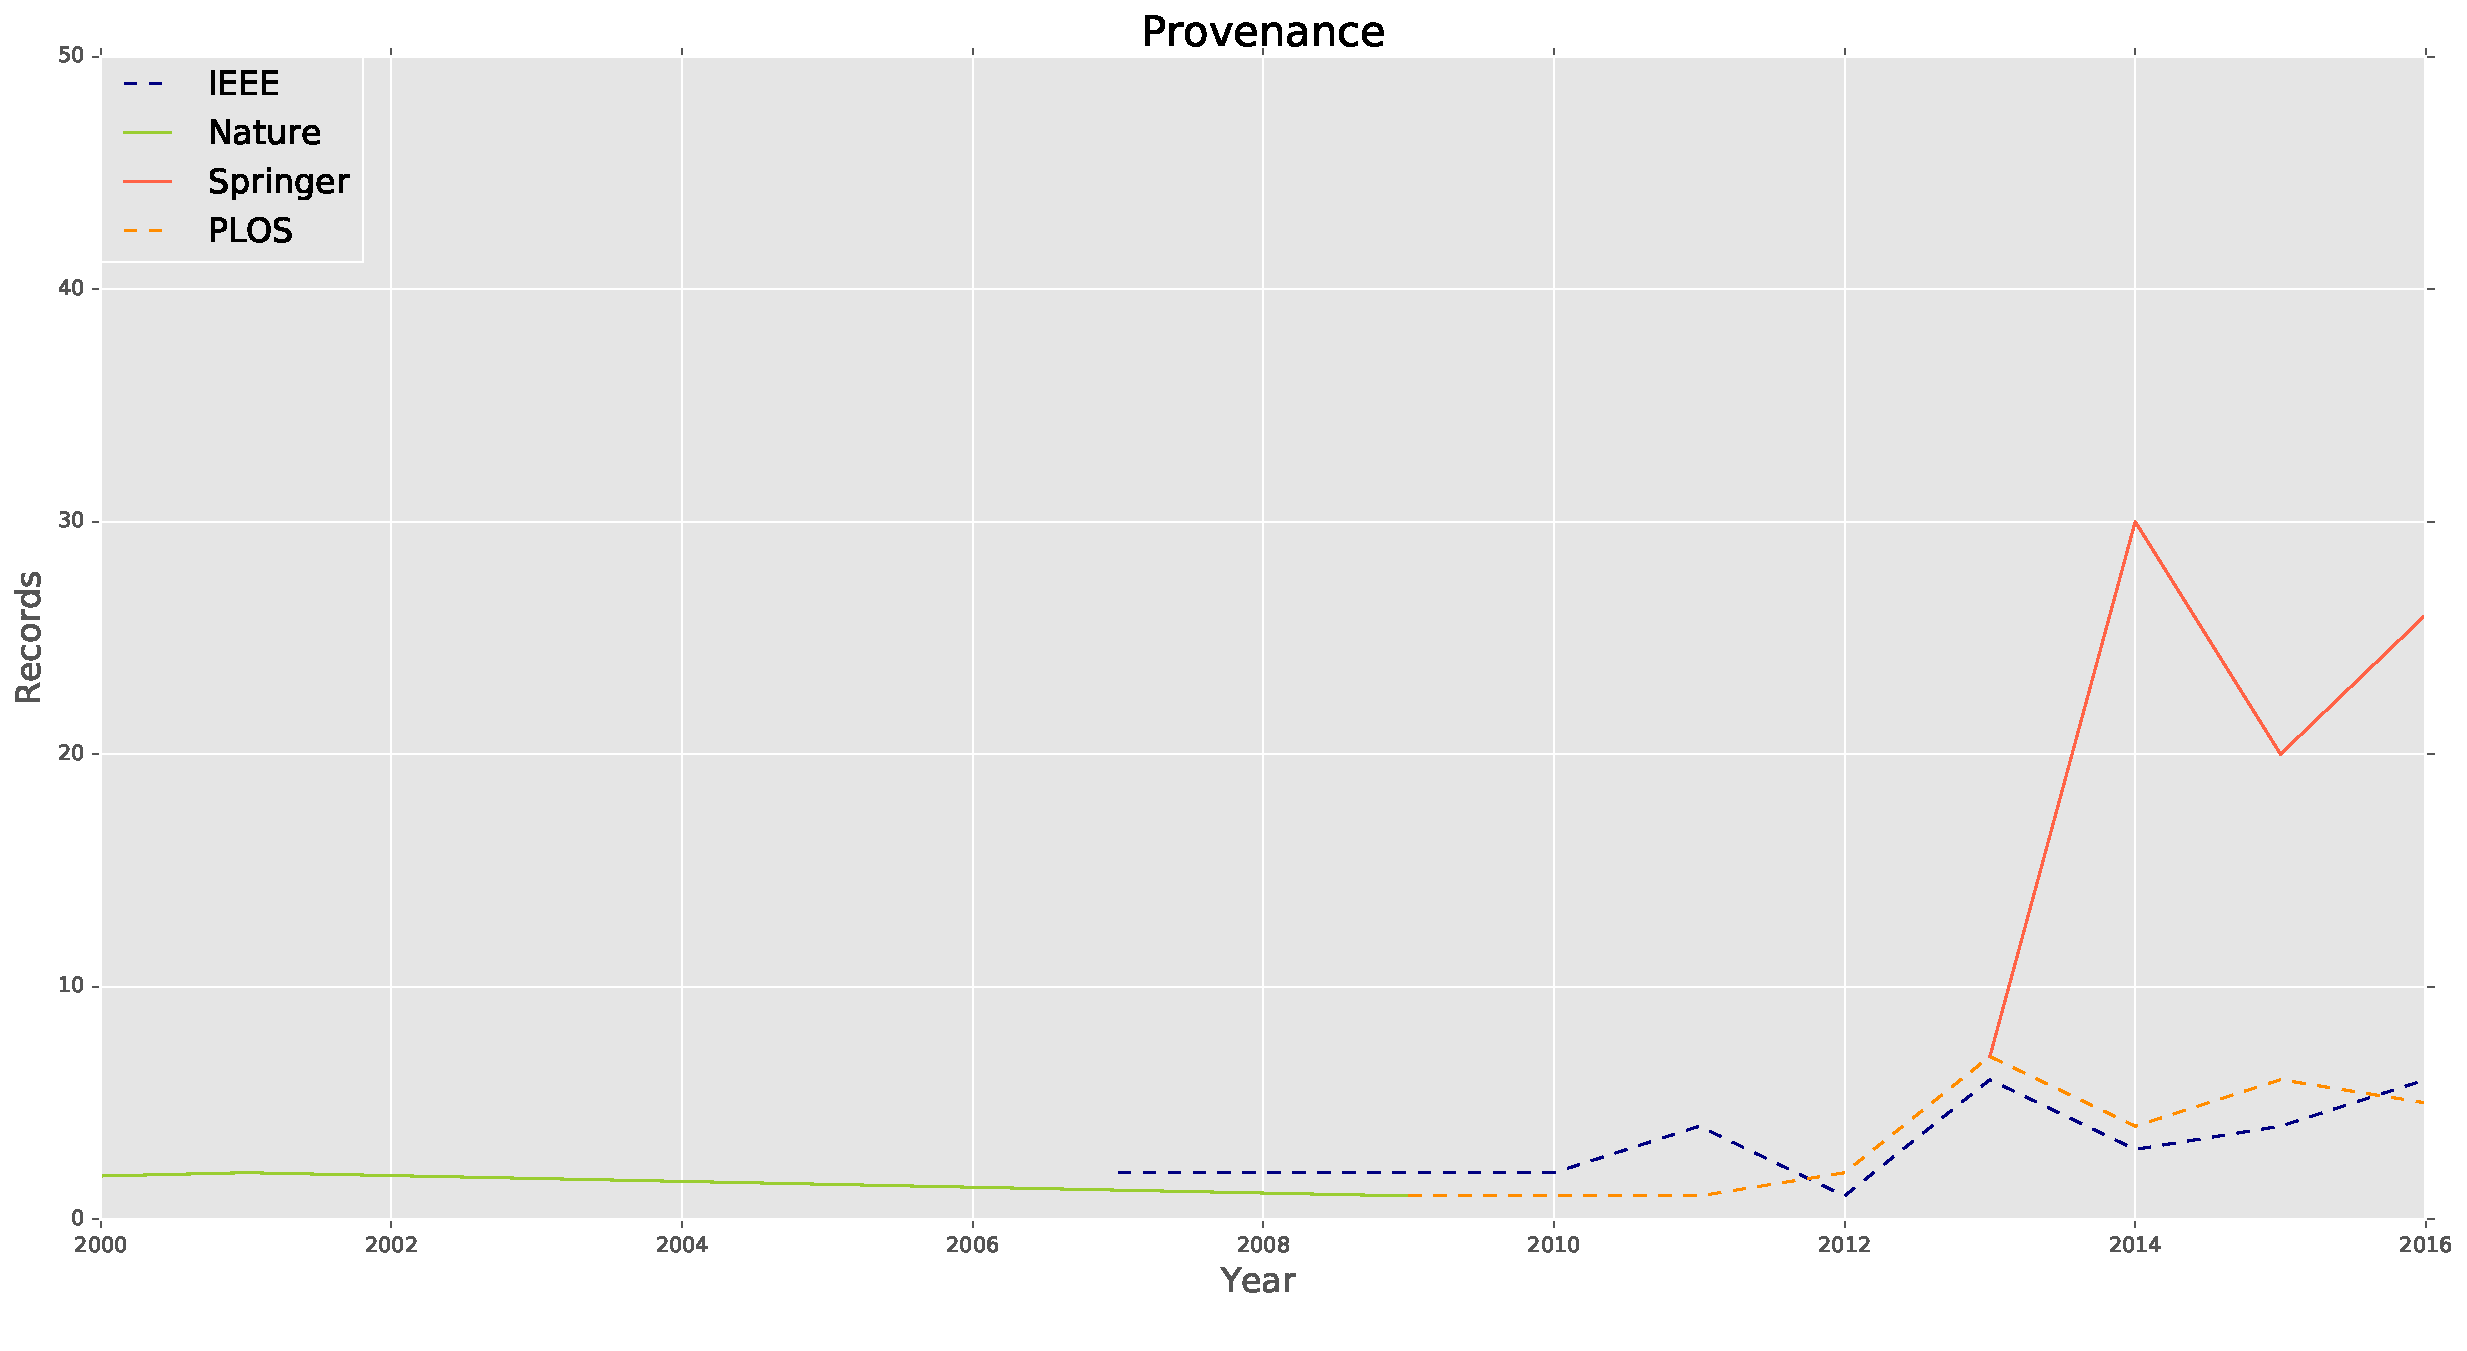
\includegraphics[width=\textwidth]{static/provenance.pdf}
\end{center}
\end{frame}

\begin{frame}
\begin{center}
\begin{figure}[H]
    \documentclass{standalone}

\usepackage{tikz}
\usepackage{standalone}
\usetikzlibrary{calc}
\usetikzlibrary{decorations.pathmorphing}
\usetikzlibrary{fit}                    % fitting shapes to coordinates
\usetikzlibrary{backgrounds}    % drawing the background after the foreground

\tikzstyle{background}=[orange, rectangle, draw, inner sep=0.2mm,
           rounded corners=1mm, ultra thick]

\begin{document}
\begin{tikzpicture}

\tikzstyle{state}=[minimum width=0.4cm, font=\boldmath];
    

    \node[ultra thick, draw=orange] (0) at (0, 0) [state] {tools.py};
    \node[ultra thick, draw=orange] (1) at (0, -2) [state] {doc/};

    \node[ultra thick, draw=orange] (2) at (0, -4) [state] {arcas.readthedocs.io/};

    \node[ultra thick] (3) at (4, 0) [state] {ieee};
    \node[ultra thick] (4) at (6, 0) [state] {nature};
    \node[ultra thick] (5) at (4, -1) [state] {arxiv};
    \node[ultra thick] (6) at (6, -1) [state] {$\dots$};  

    \node [background, inner sep=4mm, fit=(3) (4) (5) (6)] {};

    \node[ultra thick] (7) at (4, -3) [state] {test{\_}ieee};
    \node[ultra thick] (8) at (6, -3) [state] {test{\_}nature};
    \node[ultra thick] (9) at (4, -4) [state] {test{\_}arxiv};
    \node[ultra thick] (10) at (6, -4) [state] {$\dots$};  

    \node [background, fit=(7) (8) (9) (10)] {};

    \draw (1) edge[out=-90, in=90, -, thick, dotted] node [above] {} (2);

    \node [background, brown, inner sep=8mm, fit= (0) (1) (2) (3) (4) (5) (6) (7) (8) (9) (10)] {};

\end{tikzpicture}
\end{document}
\end{figure}
\end{center}
\end{frame}

\begin{frame}
\begin{center}
\begin{figure}[]
        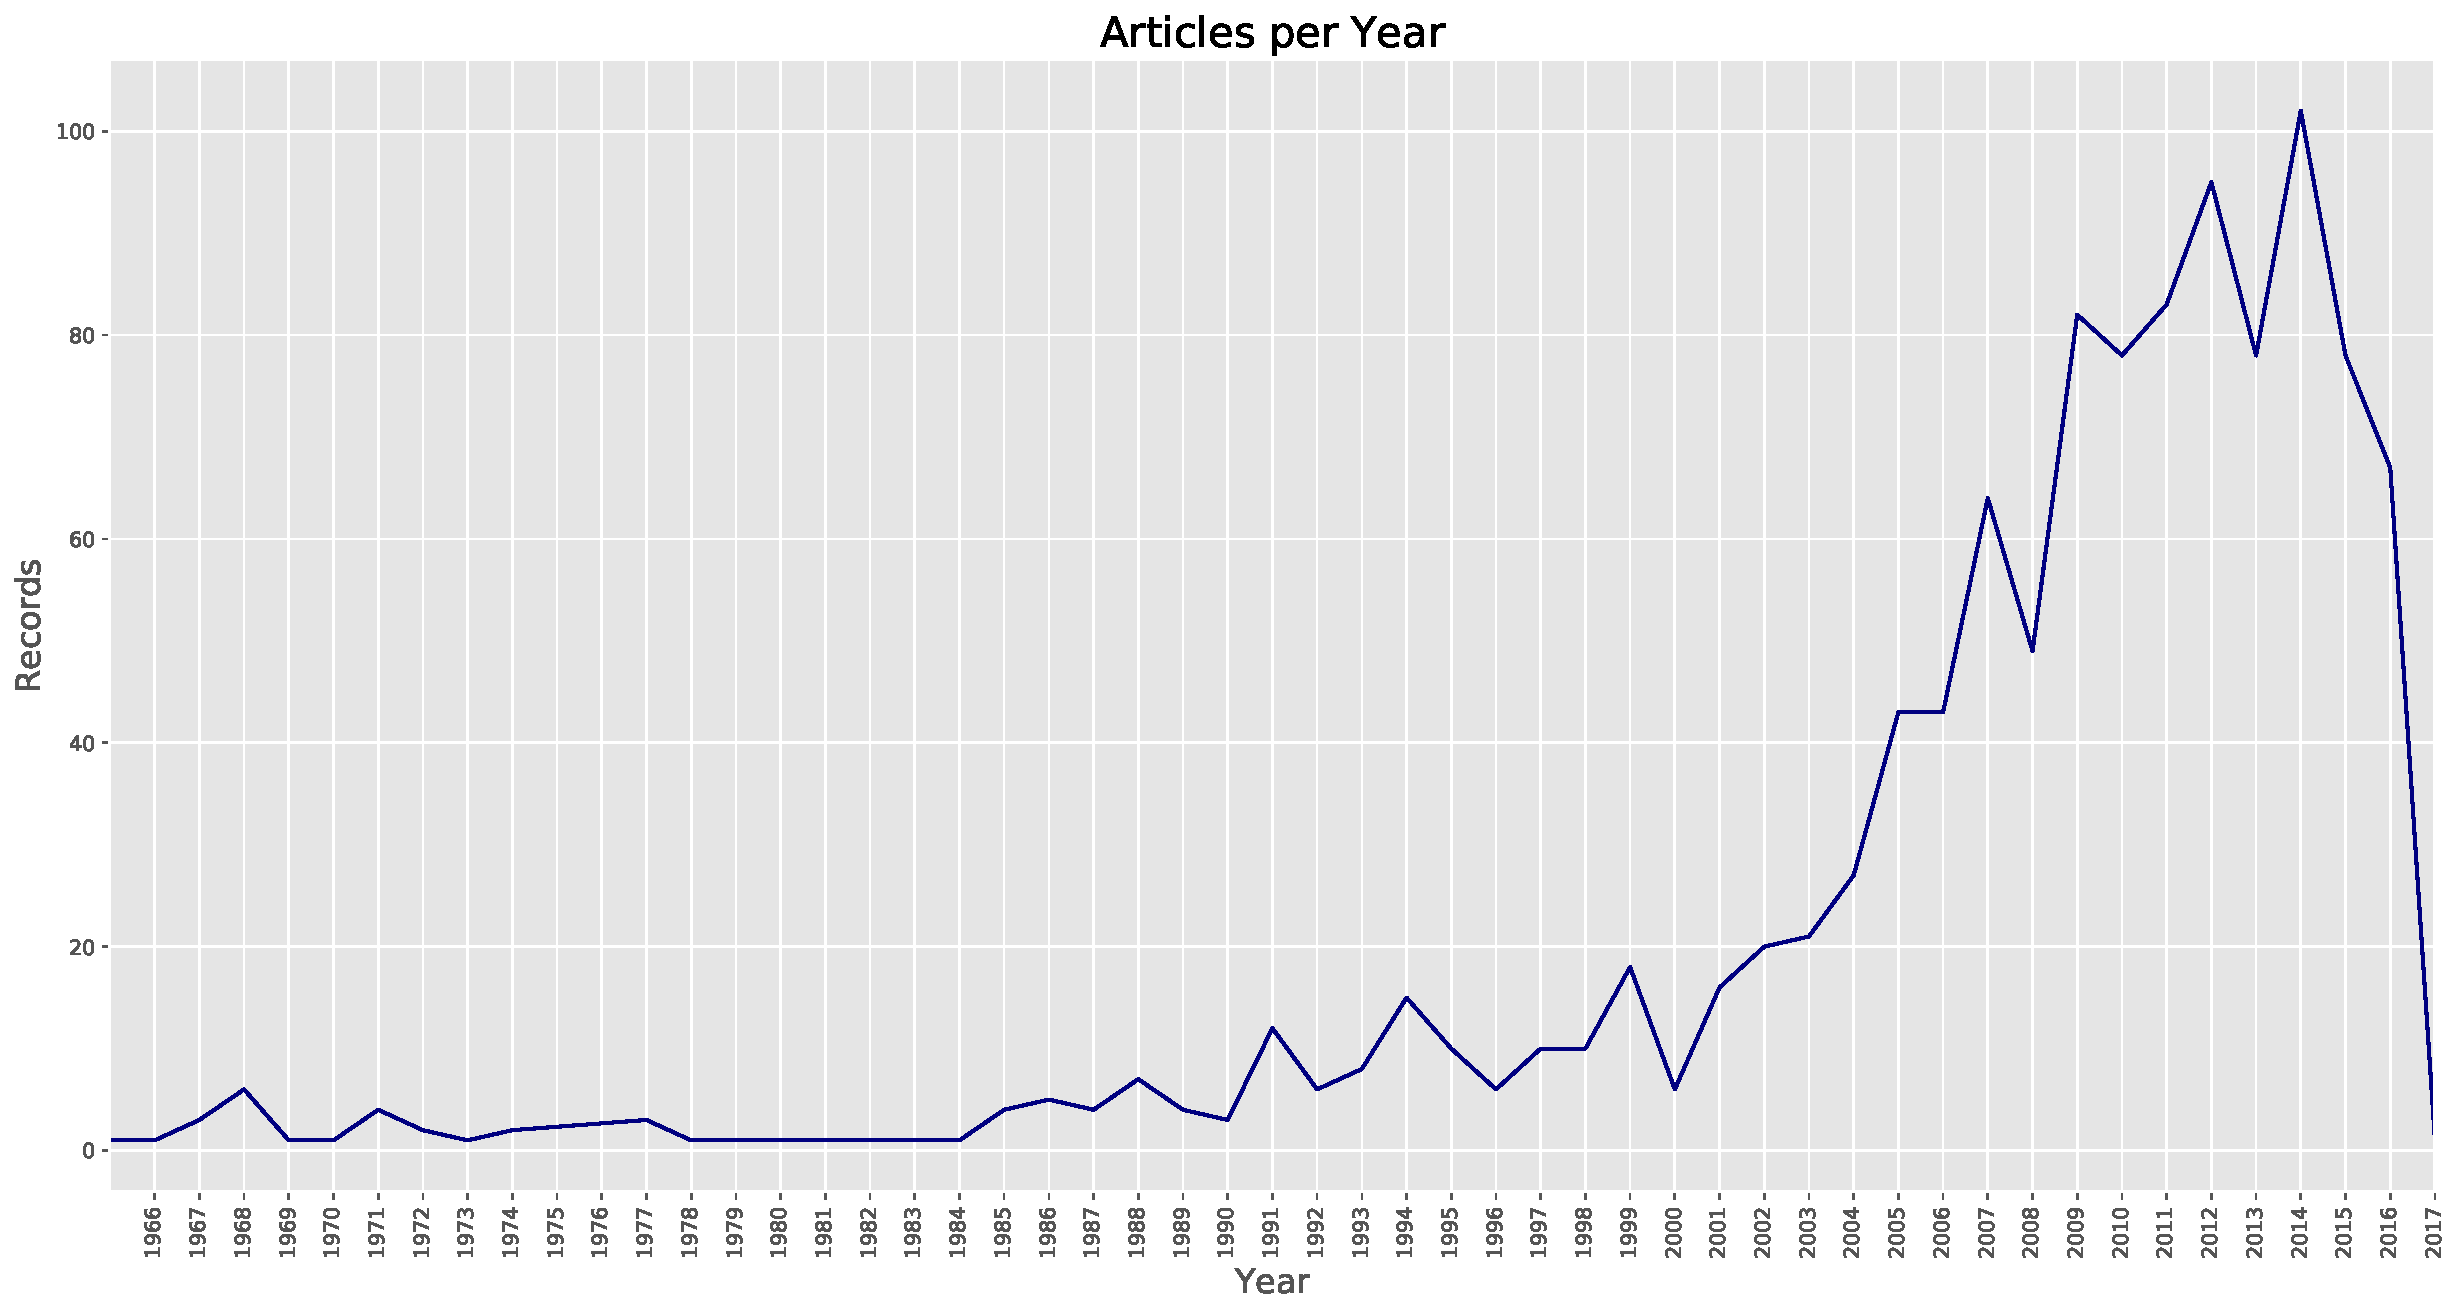
\includegraphics[width=\textwidth]{static/articles-year.pdf}
\end{figure}
\end{center}
\end{frame}

\begin{frame}
\begin{center}
\begin{figure}[]
        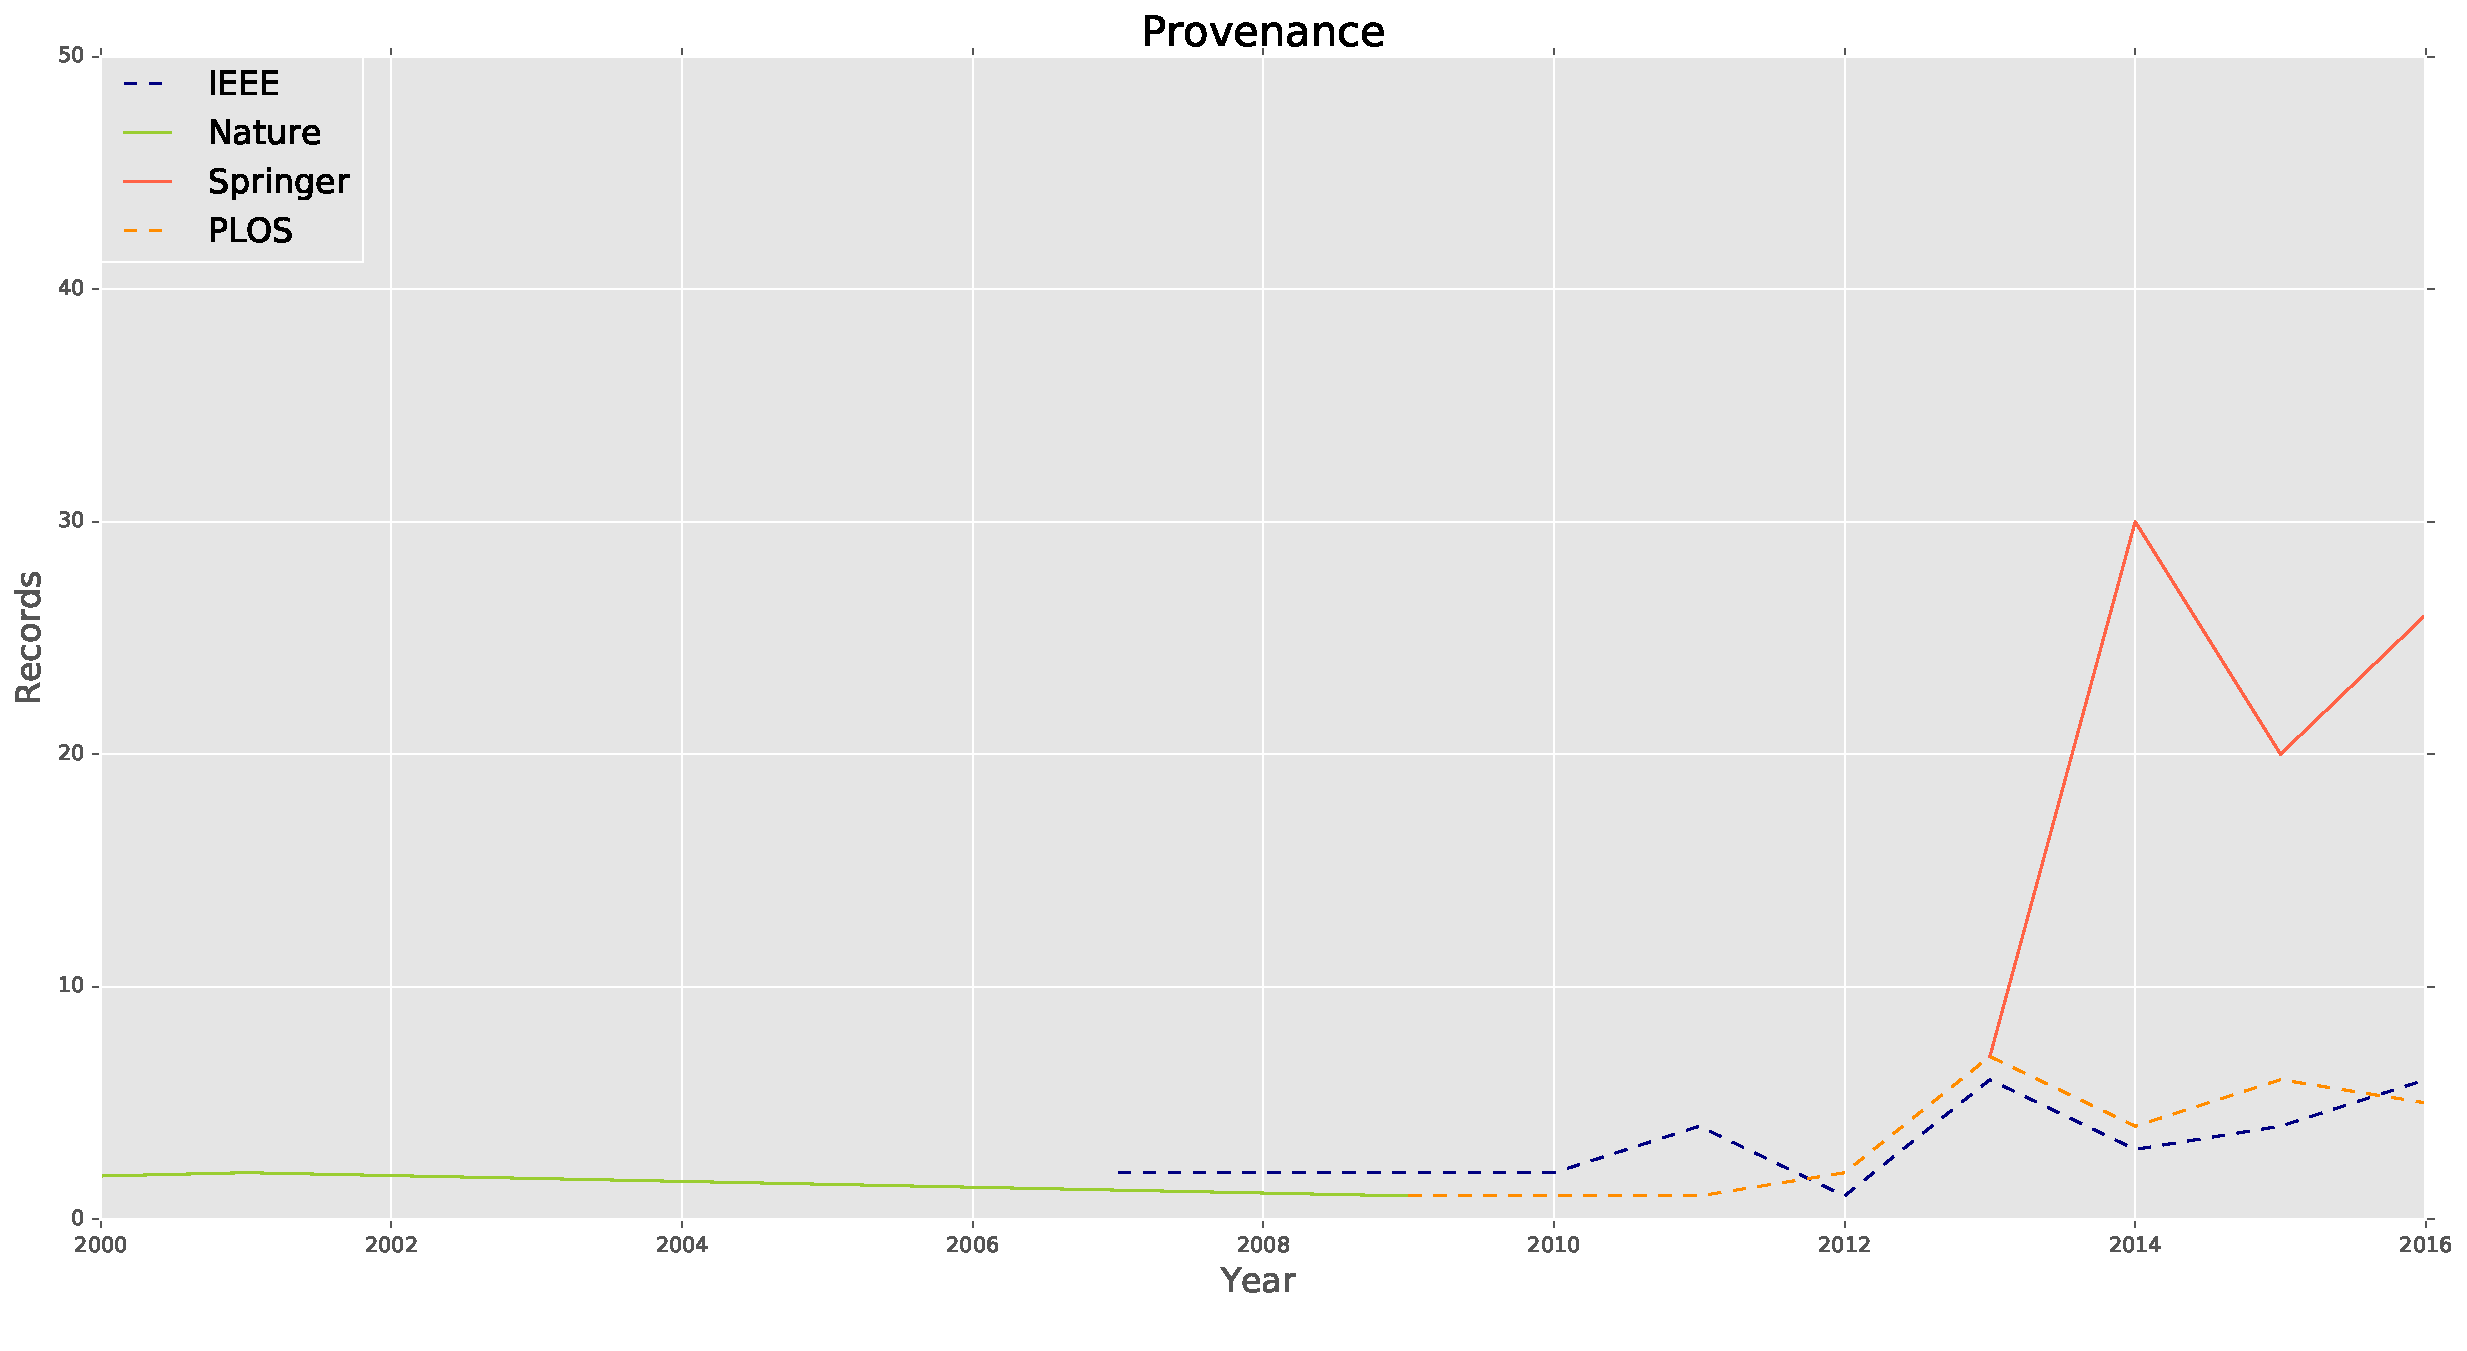
\includegraphics[width=\textwidth]{static/provenance.pdf}
\end{figure}
\end{center}
\end{frame}

\begin{frame}
\begin{center}
\begin{figure}[]
        \includegraphics[width=\textwidth]{static/network.pdf}
\end{figure}
\end{center}
\end{frame}


\begin{frame}[fragile]
    \begin{minted}
    [
    framesep=2mm,
    baselinestretch=1.2,
    bgcolor=DarkGray,
    fontsize=\footnotesize,
    ]
    {python}
 arcas_scrape -p ieee -t "Prisoner Dilemma" -a "Nowak" -y 2014
 ... -r 1 -s 2
    \end{minted}
    \hspace{10mm}
    \begin{minted}
    [
    framesep=2mm,
    baselinestretch=1.2,
    bgcolor=DarkGray,
    fontsize=\footnotesize,
    ]
    {python}
 arcas_scrape -p ieee -b "game theory" -t "Prisoner Dilemma"
 ... -a "Nowak" -y 2014 -r 1 -s 2
    \end{minted}
\end{frame}

\begin{frame}
	\begin{center}
		\huge{\textbf{}}\\~\\
		\small{@NikoletaGlyn}\\
		\small{https://github.com/Nikoleta-v3}\\
		\small{ttps://github.com/Nikoleta-v3/Arcas}
	\end{center}
\end{frame}

\end{document}




